\chapter{Introduction}



\section{Modeling genomes} % (fold)
\label{sub:modeling_genomes}

Multichromosomal genomes are represented using a notation as in previous work~\cite{Bergeron2006}.\\
A chromosome is represented by a sequences of genes.
If the chromosome is \emph{linear} it is flanked by \emph{telomeres} ($\circ$).
A genome $G$ is the set of its chromosome.
A gene $g$ from $G$ has two extremeties, the tail ($g^t$) and the head ($g^h$).
Since genes can be located both DNA strands, we encode this by a leading $-$, i.e. $g$ is located on the leading strand and $-h$ on the lagging strand.
It is possible to describe \emph{adjacencies} between two genes $g$ and $h$. 
If $g$ and $h$ are two consecutive genes in the genome $G$, we can describe their adjacency by their adjacent gene extremeties.
Note that there exist four different ways of orientation for two genes.
Gene extremeties that are located on the end of a linear chromosome are often combined with the telomere, thus forming a \todo{Rausstreichen} \emph{telomeric adjacency}. 
In order to describe a genome $G$ it is possible to use the set of chromosomes or the set of adjacencies $A$.\\
The genome $G_A$ in Figure~\ref{fig:genomeRep} has two linear chromosomes with five genes, where $G_A=\{(\circ\ 1\ -2\ 3\ \circ),(\circ\ 4\ 5\ \circ)\}$
and $A=\{\circ 1^t, 1^h2^h, 2^t3^t, 3^h\circ, \circ 4^t, 4^h5^t, 5^h\circ\}$\\ \ \\

\begin{figure}[h]
	\centering
	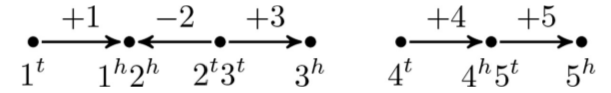
\includegraphics[scale=0.4]{figures/genomeRep.png}
	\caption{%
	 The Genome $G_A=\{(\circ\ 1\ -2\ 3\ \circ),(\circ\ 4\ 5\ \circ)\}$ with its corresponding adjacency set 
	 $A=\{\circ 1^t, 1^h2^h, 2^t3^t, 3^h\circ, \circ 4^t, 4^h5^t, 5^h\circ\}$.  
	 Figure taken from~\cite{Feijao2015}
		}%
	\label{fig:genomeRep}
\end{figure}
\noindent
Given two genomes $A$ and $B$ with the same set of genes, the \emph{breakpoint graph} $BP(A,B)$ is defined in the following way~\cite{Tannier2009}:\\
Let $G=BP(A,B)$ be a graph where the vertex set $V(G)$ is the set of gene extremities and the edge set $E(G)$ the set of non-telomeric
adjacencies of $A$ and $B$.
The edges are also called \emph{A-edges} and \emph{B-edges} respectively. \\ \ \\
It is common to draw the adjacencies from $A$ and $B$ in different colors within the breakpoint graph.
Each component in $BP(A,B)$ is either a cycle, an even path or an odd path.
The parity of a path is defined by the \emph{size} of a component, where the size is the number of vertices in the component.\\
An example for a breakpoint graph $BP(A,B)$ with two genomes $A$ and $B$ is given in Figure~\ref{fig:BPgraph}.

\begin{figure}[h]
	\centering
	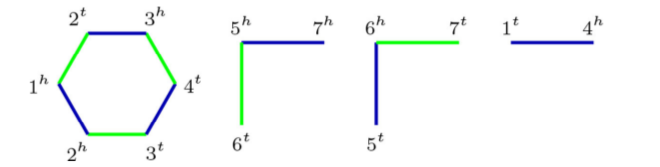
\includegraphics[scale=0.5]{figures/BPG_1.png}
	\caption{%
		Breakpoint Graph $BP(A,B)$ of $A=\{\circ 1^t,1^h2^t,2^h3^t,3^h4^t,4^h\circ,\\\circ 5^t,5^h6^t,6^h7^t,7^h\circ\}$ and 
		$B=\{1^h2^h,2^t3^h,3^t4^t,4^h1^t,\circ 6^t,6^h5^t,5^h7^h,7^t\circ\}$.
		A-edges are green, B-edges are blue. Figure taken from~\cite{Feijao2015}.
	}%
	\label{fig:BPgraph}
\end{figure}

% section modeling_genomes (end)

\section{DCJ model} % (fold)
\label{sub:dcj_model}
The \emph{Double-Cut-and-Join} (DCJ) operation rearranges the order of genes by cutting two adjacencies and rejoining the affected extremities
in another way.
It is shown that the DCJ distance $d(A,B)$ for two genomes $A$ and $B$ can be determined using the Breakpoint Graph $BP(A,B)$~\cite{Bergeron2006}:
\[
	d(A,B) = n - c - \frac{o}{2}
\]
where $n$ is the number of genes, $c$ and $o$ are the number of cycles and odd paths in the Breakpoint Graph, respectively.\\
It is also shown that each \emph{component} can be considered independently in order to calculate the DCJ distance~\cite{Stoye2010}.\\

% section dcj_model (end)

\section{Circular Breakpoint Graph} % (fold)
\label{sub:circular_breakpoint_graph}
In order to simplify the calculation of the \emph{DCJ-distance} the Breakpoint Graph is extended to a \emph{Circular Breakpoint Graph}~\cite{Feijao2015}.
For each odd and even path in $BP(A,B)$ telomeres are added and connected in a way, such that each \emph{telomeric adjacency} in the Breakpoint Graph
is connected to a telomere. Please reconsider the example of a Breakpoint Graph in Figure~\ref{fig:BPgraph}.
The extended version to the Circular Breakpoint Graph is shown in Figure~\ref{fig:cBPgraph}.

\begin{figure}[h]
	\centering
	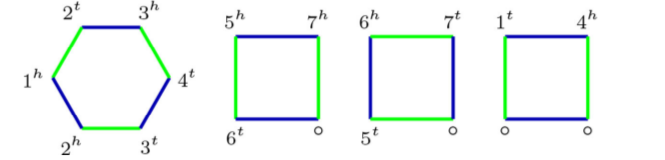
\includegraphics[scale=0.5]{figures/cBPG.png}
	\caption{%
	 Circular BP graph of the BP(A,B) from Figure~\ref{fig:BPgraph}. \emph{A-edges} are drawn in green, \emph{B-edges} are drawn in blue.
	 Figure taken from~\cite{Feijao2015}.
	}%
	\label{fig:cBPgraph}
\end{figure}

During the rest of this thesis the term Breakpoint Graph or $BP(A,B)$ refers to the circular version.